\chapter{Proof of space}
\label{ch:pospace}

\section{Introduction}

La \emph{preuve d'espace} (ou \emph{proof of space} en anglais) est un algorithme de consensus similaire à la preuve de travail à la différence qu'au lieu d'effectuer des calculs pour trouver une preuve satisfaisante, les mineurs appelés farmers vont générer des preuves pour un challenge donné à partir de données allouées sur leurs disques durs. 

Il existe principalement deux constructions pour faire du proof of space : une basée sur \textbf{l'inversion de fonctions de hachage} \cite{DBLP:conf/asiacrypt/AbusalahACKPR17} et une basée sur des \textbf{graphs acycliques orientés} \cite{DBLP:conf/crypto/DziembowskiFKP15}.

Pour ce travail, il a fallu faire un choix d'un algorithme à implémenter. Ce choix c'est porté sur l'inversion des fonctions de hachage car il y plus de ressources disponibles et la construction est plus simple à implémenter comparé aux graphs.

Ce chapitre explique le fonctionnement général du protocole tiré de la blockchain Chia.

\section{Protocole}

Dans un premier temps, les données sont générées par le farmer dans une étape appelée \textbf{plotting}. Ce sont des données pseudo-aléatoires qui ne représentent rien de particulier. D'autres algorithmes pour stocker des données utiles existent comme \emph{proof of catalytic space} ou \emph{proof of replication} utilisés dans la blockchain \href{https://filecoin.io/}{Filecoin} par exemple.

En suite, un farmer peut prouver qu'il a bien les données qu'il dit avoir stockées en trouvant une ou plusieurs preuves répondant à un challenge donné. C'est l'étape du \textbf{farming}.

Lors de la \textbf{vérification}, le vérificateur récupère la prevue, vérifie si elle est valide et est à partir de celle-ci, recalcule le challenge et vérifie s'il correspond à celui envoyé précédemment.

Proof of space est un protocole dans lequel il y a :

\begin{enumerate}
  \item un vérificateur qui envoie un challenge à un farmer et
  \item un farmer qui peut prouver au vérificateur qu'il a bien alloué la quantité d'espace spécifiée à un instant $t$.
\end{enumerate}

\begin{figure}[H]
  \centering
  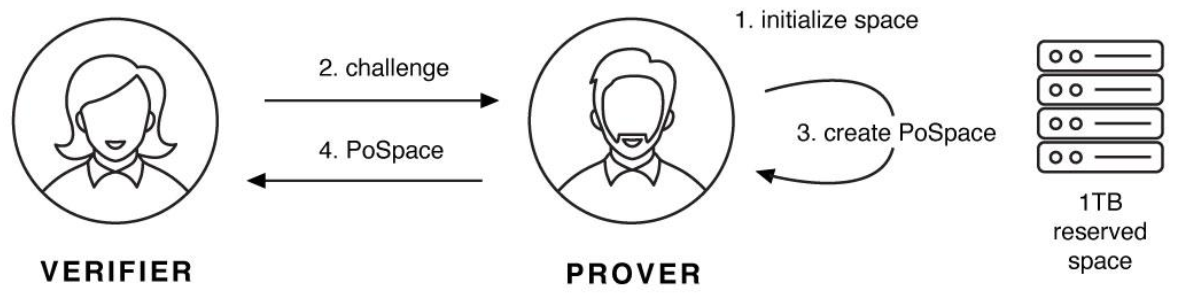
\includegraphics[width=\textwidth]{images/pospace.png}
  \caption{Diagramme du protocole \emph{proof of space} montrant les différentes étapes. Tiré de \cite{chia:consensus}}
\end{figure}

\subsection{Plotting}

Le plotting est un procédé non-interactif durant le lequel le farmer va créer les données, appelées \textbf{plots}, qui seront stockées et qui permettront de trouver les preuves d'espace liées aux challenges. Ce procédé peut être long, cela peut prendre de plusieurs heures à plusieurs jours suivant la quantité de données allouées.

La construction de cette preuve d'espace est basée sur la construction de Chia \cite{chia:construction}, elle-même basée sur l'inversion de fonctions de hachage \cite{DBLP:conf/asiacrypt/AbusalahACKPR17}.

Le principe est le suivant: le vérificateur donne une fonction $f: N \rightarrow N$ avec $N = \{0,1\}^k$ et $k$ le \textbf{space parameter}, modélisée comme un oracle aléatoire, au farmer, puis, lors de la vérification, demande au farmer l'entrée correspondant à une sortie choisie aléatoirement. Le farmer a alors besoin d'inverser rapidement la fonction. Pour ce faire, on peut imaginer que le farmer précalcule les sorties de la fonctions. Ainsi, lorsqu'un challenge est donné au farmer, il a simplement à regarder dans la table des valeurs de sortie par une recherche dichotomique (les données $(f(x), x)$ sont triées par $f(x)$) et renvoyer l'entrée associée comme avec une lookup-table. En pratique, on utilisera une \gls{hash-function}. La table serait alors donnée par $f(x) = H(n\|x)$, avec $n$ un nonce aléatoire.

\begin{figure}[H]
  \centering
  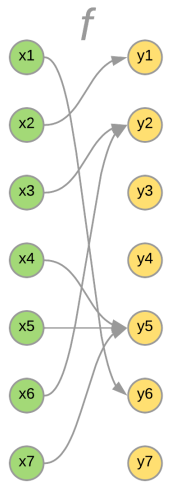
\includegraphics[width=3.5cm]{images/pospace_1.png}
  \caption{Table simplifiée, tiré de \cite{chia:construction}}
\end{figure}

Cependant, à cause d'un compromis temps-mémoire expliqué par \emph{Martin Hellman} en 1980, il est possible de faire une attaque avec laquelle il est possible de stocker uniquement $\sqrt{2^k}$ valeurs et de calculer uniquement $\sqrt{2^k}$ valeurs à la demande. L'attaque de Hellman part du principe que la fonction en question est facile à calculer. Chose qui n'est pas nécessaire quand on veut faire du proof of space puisque l'on veut juste pouvoir générer des preuves rapidement et les vérifier rapidement. La génération peut prendre du temps car elle ne sera faite qu'une fois. Ainsi, pour éviter un maximum ce problème, il faut rendre la fonction $N \rightarrow N$ \textbf{difficile à calculer} pour rendre l'initialisation plus longue et réduire le compromis temps-mémoire mais elle doit rester facilement inversible, ceci pour forcer les farmers à stocker l'entièreté de la table.

Pour la rendre plus difficile à calculer, on peut modéliser une nouvelle fonction $f(x_1)=f_2(x_1,x_2)$, où $f_2(x_1,x_2)=H(x_1\|x_2)$ avec \textbf{la condition} que $f_1(x_1)=f_1(x_2)+1$, avec $f_1$ également une fonction de hachage. Ainsi, à partir d'un challenge $z$, le farmer doit trouver les valeurs $x_1$ et $x_2$. Et comme la fonction $f$ n'est pas facilement calculable, le farmer doit stocker toutes les tables pour pouvoir répondre rapidement. Cette construction, illustrée ci-dessous, est toujours vulnérable aux attaques de Hellman mais plus ajoute de fonctions (donc de tables), plus on rend la génération des tables lente diminuant le compromis temps-mémoire. Chia utilise 7 tables.

\begin{figure}[H]
  \centering
  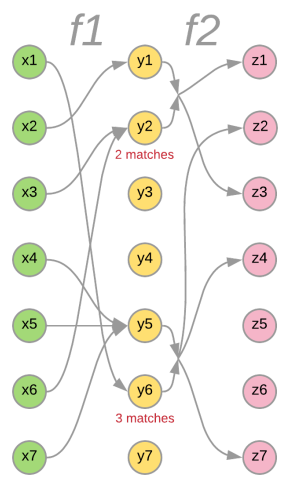
\includegraphics[width=6cm]{images/pospace_2.png}
  \caption{3 tables générées à partir de 2 fonctions, tiré de \cite{chia:construction}}
\end{figure}

Ainsi, le farmer choisi un nombre $k$, le \emph{space parameter} pour définir combien il souhaite allouer d'espace. Il génère également une \emph{plot seed}, utilisée lors de la génération de la première table afin de rendre les données uniques. La plot seed joue le rôle d'une nonce lors de l'initialisation. La quantité de données finale sera exponentielle par rapport au nombre $k$. Le temps de la génération dépend lui de la puissance de l'ordinateur effectuant le plotting puisqu'il s'agit principalement d'exécution de fonctions de hachage comme vu précédemment. C'est donc le CPU qui sera beaucoup sollicité durant cette étape. 

Chaque table contiendra environ $2^k$ entrées et chaque entrée d'une $\textsf{table}_i$ pointera vers 2 entrées dans la $\textsf{table}_{i-1}$. La première table quant à elle contiendra ce qu'on appellera les \emph{x-values}. Ce sont simplement des nombres entiers de $0$ à $2^k-1$. A noter que ce processus à besoin de plus d'espace de stockage que souhaité pour le plot final car il générera des données qui seront ensuite nettoyées et compressées. On supprimera ensuite les sorties des fonctions de hachages de chaque table intermédiaire pour ne stocker plus que les index dans la 1ère table pour chaque table.

Une fois les tables générées, on peut commencer à faire du \textbf{farming}.

\subsection{Farming}

Le \emph{farming} est le processus dans lequel le farmer reçoit un challenge et produit une preuve composé de 64 nombres entiers pour démontrer qu'il a bien alloué l'espace indiqué. Le challenge est une valeur de 256 bits (un hash par exemple). Pour ce faire, le farmer parcours la dernière table de son plot pour voir s'il trouve une entrée correspondant au challenge tel que $\underset{k}{\mathrm{trunk}}(\mathrm{Chall})=\underset{k}{\mathrm{trunk}}(\mathrm{table_4}[i])$, pour $i \in \{0,1,\dots,2^k-1\}$. S'il trouve une correspondance, le farmer parcours les tables dans le sens inverse, pour retrouver les x-values. Il renvoie ensuite les 64 valeurs au vérificateur.

Une preuve $\pi$ possède le format suivant avec la construction de Chia \cite{chia:construction} comportant 7 tables :

$\pi_{\textrm{Chall, plot\_seed, k}}=x_1, x_2, x_3, \dots, x_{64}$ (avec $x_i \in \{0, \dots, 2^k-1\}$) avec les conditions suivantes :

\begin{gather*}
  \match(f_1(x_1), f_1(x_2)), \match(f_1(x_3), f_1(x_4)), \dots \\
  \match(f_2(x_1, x_2), f_2(x_3, x_4)), \match(f_2(x_5, x_6), f_2(x_7, x_8)), \dots \\
  \match(f_3(x_1, x_2, x_3, x_4), f_3(x_5, x_6, x_7, x_8)), \match(f_3(x_9, x_{10}, x_{11}, x_{12}), f_3(x_{13}, x_{14}, x_{15}, x_{16})), \dots \\
  \match(f_4(x_1, \dots, x_8), f_4(x_5, \dots, x_{16})), \match(f_4(x_{17}, \dots, x_{24}), f_4(x_{25}, \dots, x_{32})), \dots \\
  \match(f_5(x_1, \dots, x_{16}), f_5(x_{17}, \dots, x_{32})), \match(f_5(x_{33}, \dots, x_{48}), f_5(x_{49}, \dots, x_{64})) \\
  \match(f_6(x_1, \dots, x_{32}), f_6(x_{33}, \dots, x_{64})) \\
  \underset{k}{\mathrm{trunk}}(Chall)=\underset{k}{\mathrm{trunk}}(f_7(x_1, \dots, x_{64}))
\end{gather*}

Chaque fonction $\mathsf{M}$ ci-dessus retourne << vrai >>.

Dans le cas d'une blockchain, le système est non-interactif. La preuve doit pouvoir être vérifiée par n'importe qui à tout moment sans avoir besoin de demander quoi que ce soit au farmer en question. Pour ce faire le challenge doit être généré à partir d'un élément public, par exemple le hash du dernier bloc de la chaîne. Le nonce utilisé lors de l'initialisation est dans notre cas dérivé de la clé public du farmer et envoyé avec le preuve pour pouvoir être vérifiée par tout le monde.

\subsection{Vérification}

La vérification consiste à valider une preuve donnée par un farmer. Elle est simple puisqu'il suffit de recalculer à partir ces 64 x-values et de la clé publique du farmer les valeurs des hashs, vérifier qu'ils matchent entre eux et que le dernier hash correspond au challenge.

Voici un exemple avec 4 tables et 8 \emph{x-values}. La validateur va executer les fonctions de la manière suivante :

\begin{gather*}
  f_1(x_1), f_1(x_2), f_1(x_3), f_1(x_4), f_1(x_5), f_1(x_6), f_1(x_7), f_1(x_8) \\
  f_2(x_1,x_2), f_2(x_3,x_4), f_2(x_5,x_6), f_2(x_7,x_8) \\
  f_3(x_1,x_2,x_3,x_4), f_3(x_5,x_6,x_7,x_8) \\
  y_4 = f_4(x_1,x_2,x_3,x_4,x_5,x_6,x_7,x_8) \\
  \underset{k}{\mathrm{trunk}}(y_4)=\underset{k}{\mathrm{trunk}}(\mathrm{Chall})
\end{gather*}

Il va vérifier que les sorties correspondent bien, c'est-à-dire que toutes les sorties de la fonction \textsf{M} soient égales à \texttt{vrai} :

\begin{gather*}
  \mathsf{M}(f_1(x_1), f_1(x_2)),\mathsf{M}(f_1(x_3), f_1(x_4)),\dots \\
  \mathsf{M}(f_2(x_1,x_2),f_2(x_3,x_4)),\mathsf{M}(f_2(x_5,x_6),f_2(x_7,x_8)) \\
  \mathsf{M}(f_3(x_1,x_2,x_3,x_4), f_3(x_5,x_6,x_7,x_8))
\end{gather*}

Avec la fonction $\mathsf{M}(y_1,y_2)$ qui retourne \texttt{vrai} si et seulement $y_1 = y_2 + 1$.

Le vérificateur regarde ensuite si la valeur calculée correspond avec le challenge initial.

\section{Sécurité et attaques}

Comme vu dans le chapitre sur les protocoles de consensus, \emph{proof of space} a des avantages écologiques puisque le calcul n'est réalisé qu'une fois au début lors de la génération du plot. Cela signifie que la génération de preuves ne requiert que très peu de puissance calcul et que par conséquent elle peut être exécutée rapidement à la différence de proof of work. Cela implique qu'un attaquant peut forger des blocs en avance, générer leur preuve respective et les broadcaster sur le réseau. Si ces blocs sont valides ils pourraient être acceptés par le réseau qui se base automatiquement sur la plus longue chaîne de blocs. Il y aurait du coup la possibilité pour des attaquant d'effectuer des actes de double dépenses. C'est ce que Chia appelle les \emph{Grinding attacks}.

Il y a plusieurs types de grinding attacks présentées dans leur \emph{Chia Green Paper} \cite{chia:greenpaper} :

\begin{itemize}
  \item \textbf{Digging attacks}: Si on reprend l'exemple de proof of work, un mineur sélectionne un certain nombre de transactions à inclure dans le prochain bloc pour ensuite essayer de trouver la preuve de travail correspondante. Cependant, rien ne l'empêche techniquement de calculer plusieurs challenges à la fois en prenant par exemple des transactions différentes pour maximiser ses chances de trouver une preuve. Mais cela implique que le mineur doit diviser sa puissance de calcul, ce qui ne sert donc pas à grand chose car il n'aura aucun avantage à le faire.
  
  Mais avec \emph{proof of space} ce n'est pas la même situation. Comme les preuves peuvent être générée pour un challenge sans puissance de calcul particulière, un farmer peut tenter de trouver un maximum de preuves pour plusieurs challenges et garder seulement la preuve qui a le plus de chance d'être acceptée par le réseau. Ce qui leur permettrait de gagner face à des farmers honnêtes.
  \item \textbf{Double dipping attacks}: Ici, le farmer attaquant va essayer de trouver des preuves pour plusieurs blocs différents à la fois. Normalement, le mineur/farmer doit, selon le protocole, tenter d'étendre uniquement la chaîne la plus longue. Avec proof of work, les \emph{double dipping attacks} n'existent pas pour les mêmes raison qu'il n'y a pas de \emph{digging attacks}. Mais, à nouveau, comme on peut générer des preuves efficacement avec PoSpace, il est possible n'étendre autant de branches ce le souhaite le farmer. Ce qui pose un problème pour atteindre le consensus sur quelle chaîne est la bonne si tout le monde fait ça. 
\end{itemize}

Pour palier aux \emph{digging attacks}, la blockchain Chia associe les preuves d'espace à des \emph{preuves de temps} (proofs of time) basées sur des \emph{Verifiable Delay Functions} afin de vérifier qu'un certain temps c'est réellement écoulé. Ces fonctions particulières prennent un temps réel à s'exécuter et ne peuvent pas être parallélisées. Par contre la vérification de la preuve de temps est elle réalisable rapidement. Techniquement, la blockchain utilise des exponentiations répétées sur des groupes d'ordre inconnus \cite{DBLP:conf/crypto/BonehBBF18} \cite{DBLP:conf/innovations/Pietrzak19a} \cite{DBLP:conf/eurocrypt/Wesolowski19}. Ces deux systèmes de preuves sont utilisés de manière à éviter les grinding attacks en séparant la blockchain en deux chaînes parallèles. Une chaîne appelée << trunk >> dite \emph{ungrindable} contenant uniquement les preuves d'espace et de temps et une chaîne appelée << foliage >> contenant les données des transactions.

Pour palier aux \emph{double dipping attacks}, Chia réalise en fait un compromis autorisant les farmers à farmer les $\kappa = 3$ premiers blocs de chaque profondeur.

Malheureusement pour des raisons de temps et de complexité, il n'a pas été possible d'implémenter durant ce travail un système tel que l'a fait Chia.

Un autre problème de sécurité peut survenir avec cet algorithme si la valeur de $k$, la paramètre d'espace, est trop faible. Si c'est le cas, alors un attaquant pourrait regénérer le plot trop rapidement dû à sa petite taille. Il pourrait alors générer des plots et des preuves à la volée sans stocker de données sur disque. C'est pour cela qu'une valeur minimum est codée en dur dans le code source du protocole. Ce minimum dépend du temps qui s'écoule entre la génération des blocs. Le but étant qu'il ne doit pas être possible de générer un plot plus rapidement que le temps qui s'écoule entre 2 blocs et empêcher comme ça la génération de plots à la volée et forcer les farmer à conserver leur plot s'ils veulent continuer à générer des preuves.

\section{Consensus}

Avec \emph{proof of space}, on a un moyen de prouver qu'un farmer a, à un instant précis, alloué tant d'espace de stockage pour pouvoir trouver une preuve. Mais tout seul, \emph{proof of space} ne permet pas d'obtenir un consensus entre les nœuds comme pourrait le faire Bitcoin avec \hyperref[consensus:pow]{proof of work}. Ceci à cause des attaques présentées ci-dessus.

C'est pour cela qu'il est nécessaire d'y inclure un autre algorithme comme du \emph{proof of time} avec des VDF comme l'a fait Chia ou du \emph{proof of history} par exemple.

Voyant la complexité de leur algorithme de consensus \cite{chia:consensus}, ce travail se limite à l'implémentation du \emph{proof of space} et d'une blockchain simple.

\section{Implémentation}

Cette section présente l'implémentation du proof of space basé sur l'inversion de fonctions de hachage. L'implémentation est faite en \textbf{Rust} et est basée sur la construction de la blockchain Chia \cite{chia:construction}. A noter que dans la majorité de la construction, on travail en bits et non en octets. Chaque troncage ce fait au niveau des bits.

\subsection{Génération des tables}

L'objectif ici est de créer les données sous forme de tables de manière à pouvoir donner une ou plusieurs preuves en fonction d'un challenge donné. La construction utilise 7 tables au total. Chaque table comporte $\bigO(2^k)$ entrées. C'est-à-dire qu'il n'y a pas nécessairement $2^k$ entrées exactement. Il peut y en avoir plus ou moins.

Comme expliqué précédemment, chaque entrée pointe vers deux entrées dans la table précédente à condition qu'une \emph{matching function} $\mathsf{M}$ soit satisfaite. Ainsi une entrée dans la dernière table, la table 7, pointera vers 2 entrées dans la table 6. Chacune de ces 2 entrées pointeront vers 2 entrées dans la table 5 etc\dots jusqu'à la table 1. Donc une entrée dans la dernière table pointera indirectement vers 64 entrées dans la première table ($2^{7-1} = 64$).

La génération des tables comporte plusieurs phases. Une première phase où on génère les tables et des phases ensuite où on supprime, trie et réordonne les entrées des tables pour optimiser le stockage et la recherche. Seule la phase 1 est implémentée et sera présentée ci-dessous.

La phase 1 consiste à générer les tables de la 1 à la 7. On commence donc par la table 1. On calcule $f_1(x)$ pour $x \in \{0,\dots,2^k-1\}$. La fonction $f_1$ est simplement un ChaCha8 avec la plot seed en clé. On utilise ChaCha comme \acrshort{prng} avec un nombre réduit de rounds pour la vitesse.

\inputsourcecode{rust}{"sources/f1.txt"}{Calcule de la fonction $f_1$}

Pour simplifier la compréhension de cette fonction: les entrées sont 0, 1, 2, \dots, $2^k-1$. La sortie pour 0 sera les $k$ premiers bits du keystream. La sortie de 1 ce sera les $k$ bits suivant et ainsi de suite jusqu'à $2^k-1$. On peut remarqué qu'il y a une extension rajoutée à la fin (ligne 28-29). On rajoute ici 6 bits au keystream ce qui fait que $f_1(x)$ prend $k$ bits en entrée et sort $k+6$ bits en sortie. Ces 6 bits sont les bits de poids forts de $x$, ceci dans le but de minimiser les collisions (paradoxe des anniversaires). Le nonce lui est défini à 0. Il n'a pas d'importance puisqu'on utilise la \emph{plot seed} comme graine pour le PRNG. Cette plot seed est unique pour chaque farmer.

On stocke ensuite les entrées, les \emph{x-values} ($0,1,2,\dots,2^k-1$) accompagnées de leur valeur de sortie respective de $f_1$ sur le disque. On les trie par les valeurs de sortie pour optimiser la recherche de matchs lors du calcul de la table suivante. La table 1 est maintenant terminée et on peut passer à la table 2.

Pour construire la deuxième table, il nous faut collecter les valeurs de sortie (les $f_1(x)$) de la table 1 qui, deux par deux, satisfont la \emph{matching function}. En pratique la matching function est :

\inputsourcecode{rust}{"sources/match_naive.txt"}{Fonction de matching naïve}

Cette fonction illustre bien les conditions de match entre deux éléments mais n'est pas très performante car possède une complexité de $\bigO(6N^2)$ avec $N$ la taille d'un bucket \cite{chiapos}. Un bucket est un sous-ensemble d'une table. Pour savoir dans quel bucket se trouve une entrée on fait: $\mathsf{bucket\_id} = \lfloor\frac{y_i}{119 * 127}\rfloor$. La première condition de la matching function est que les bucket\_id des 2 entrées soient adjacents. C'est-à-dire que $\mathsf{bucket\_id_{yl}} + 1 = \mathsf{bucket\_id_{yr}}$. Cela permet de réduire les lectures sur le disque pour trouver les matchs car les éléments sont proches les uns des autres. C'est pour cela que les tables doivent être triées par les valeurs de sortie des fonctions de hachage. La deuxième condition est assez complexe. Elle sert à éviter des cycles entre les entrées si on représente l'ensemble sous forme de graph. Ces cycles peuvent être compressés ce qui représente une potentielle attaque car ça permettrait d'optimiser le stockage. C'est pour cela que les paramètres $B = 119$ et $C = 127$ ont ces valeurs. Les preuves mathématiques sont assez complexes et vont au-delà du périmètre de ce travail mais sont expliquées dans leur document de construction \cite{chia:construction}.

Ensuite, pour chaque couple $(y_1=f_1(x_1), y_2=f_1(x_2))$ tel que $\textsf{M}(y_1, y_2) = \textsf{Vrai}$, on calcule la fonction $f_2$ sur les \emph{x-values}:
\begin{equation*}
  f_2(x_1,x_2) = \underset{k + 6}{\textsf{trunk}}(\textsf{BLAKE3}(x_1\|x_2))
\end{equation*}

On stocke ensuite les sorties de $f_2$ en gardant en mémoire l'emplacement des x-values dans la table 1. Pour ce faire, et comme il y a 2 valeurs à mémoriser, on va utiliser des index dans la table 1 sous forme de << position >> et d'<< offset >>. La position est un nombre entier indiquant où se signature la première valeur ($x_1$) dans la table 1 et l'offset est aussi un nombre entier qui lui indique où la deuxième valeur ($x_2$) se situe par rapport à la première. Techniquement cela permet d'optimiser le stockage car comme les entrées sont triées par $f_1(x_i)$ et que $f_1(x_1) + 1 = f_1(x_2)$, l'offset se sera jamais très grande et peut être stocké sur moins de bits. 

Voici ci-dessous le code permettant de trouver les matchs à stocker dans la table 2 :

\inputsourcecode{rust}{"sources/core.txt"}{Calcul des matchs pour la table 2}

Dans le code ci-dessus, on utilise un version optimisée de la fonction de matching présentée précédemment. Dans un premier temps, on place les entrées de la table 1 dans un bucket gauche ou droite en fonction de leur bucket\_id (\verb|y_bucket| dans le code ci-dessus). On peut le faire avec une seule boucle car les entrées sont triée par \verb|entry.fx|. Une fois les buckets de gauche et de droite rempli, on regarde s'il y a des matchs entre les deux buckets. La fonction \verb|fx.find_matches| n'a besoin que de vérifier la deuxième condition. La première étant déjà vérifiée en plaçant correctement les entrées à droite ou à gauche.

Maintenant, pour chaque match trouvé il faut calculer $f_2(x_1,x_2)$ :

\inputsourcecode{rust}{"sources/core_f2.txt"}{Calcul de $f_2$ pour chaque match}

On peut remarquer que la fonction \verb|calculate_fn| prend en fait 3 entrées: $f_1(x_1)$ (\verb|left_entry.fx|), $x_1$ (\verb|left_entry.metadata|) et $x_2$ (\verb|right_entry.metadata|). En plus de hacher $x_1$ et $x_2$, elle va aussi hacher $f_1(x_1)$. Cela permet de s'assurer que les tables se font bien l'une après l'autre et qu'on ne saute pas de table. Ainsi on ne peut pas commencer par la table 7 et essayer de trouver des matchs, les preuves résultantes seraient refusées par le réseau qui applique le bon algorithme.

La fonction $f_2$, en plus de retourner le hash, va également retourner une version concaténée des entrées ($x_1\|x_2$) que l'on va stocker avec la sortie, la position et l'offset. Cela sera utile pour pouvoir calculer les tables suivantes. Cette concaténation également effectuée par la fonction \verb|calculate_fn| n'est simplement une concaténation car cela donnerait des données en sortie trop grande au moment de le faire sur les dernières table et limiter le nombre de bits en sortie de la concaténation permet d'obliger un attaquant souhaitant faire une attaque de Hellman à stocker des bits supplémentaires ou faire plus de recherche sur le disque \cite{chia:construction}. C'est pourquoi la \emph{collation} est tronkée à $x \times k$ bits avec $x$ qui change en fonction de la table qu'on est en train de calculer. La valeur de $x$ permet d'assurer que le compromis temps-mémoire est plus coûteux qu'en calculant de manière honnête \cite{chia:construction}. Cette \emph{collation} est stockée dans les metadatas de l'entrée pour permettre un calcul facile pour les tables suivante car ces metadatas seront utilisées comme entrée dans \verb|calculate_fn| lors du calcul de la prochaine table.

Voici ci-dessous le code de la fonction \verb|calculate_fn| :

\inputsourcecode{rust}{"sources/fn.txt"}{calculate\_fn}

Après avoir haché les 3 valeurs ensemble, on calcul la valeur de concatenation (\emph{collation}). De la table 2 à 3, c'est simplement une concatenation: $x_1\|x_2$ et $x_1\|x_2\|x_3\|x_4$. Mais ensuite, de la table 4 à 7, la valeur de la collation vaut aussi le hash que qui vient d'être calculé mais est lui tronqué à $x \times k$ bits au lieu de $k + 6$ bits.

Il faut encore trier les entrées de la table 2 par $f_2$ et la génération de la seconde table est terminée.

Il reste plus que 5 tables, mais heureusement le calcul est identique à la table 2. Il suffit de lire la table 2, trouver les matchs, calculer $f_3$ avec la même méthode (\verb|calculate_fn|) et stocker les valeurs dans la table 3. Et ainsi de suite jusqu'à la table 7.

Pour mieux visualiser, voici un tableau récapitulatif, tiré de \cite{chia:construction}, de ce que devrait contenir chaque table après cette première phase :

\begin{table}[H]
  \centering
  \begin{tabular}{l l l}
    \textbf{Table} & \textbf{Données} & \textbf{Tri} \\
    \hline
    \hline
    $\mathrm{Table_1}$ & $f_1,x$ & Trié par $f_1$ \\
    \hline
    $\mathrm{Table_2}$ & $f_2,\mathrm{pos_1},\mathrm{offset},C_3$ & Trié par $f_2$ \\
    \hline
    $\mathrm{Table_3}$ & $f_3,\mathrm{pos_2},\mathrm{offset},C_4$ & Trié par $f_3$ \\
    \hline
    $\mathrm{Table_4}$ & $f_4,\mathrm{pos_3},\mathrm{offset},C_5$ & Trié par $f_4$ \\
    \hline
    $\mathrm{Table_5}$ & $f_5,\mathrm{pos_4},\mathrm{offset},C_6$ & Trié par $f_5$ \\
    \hline
    $\mathrm{Table_6}$ & $f_6,\mathrm{pos_5},\mathrm{offset},C_7$ & Trié par $f_6$ \\
    \hline
    $\mathrm{Table_7}$ & $f_7,\mathrm{pos_6},\mathrm{offset}$ & Trié par $f_7$ \\
    \hline
  \end{tabular}
  \caption{Contenu des table 1 à 7 après la 1ère phase}
\end{table}

$C_3$ à $C_7$ sont justement les \emph{collations} calculées pour la table suivante.

\subsection{Génération de preuves}

\lipsum[1]

\subsection{Vérification de preuves}

\lipsum[1]

\section{Résultats}

\lipsum[1]

\subsection{Performances}

\begin{figure}[H]
  \centering
  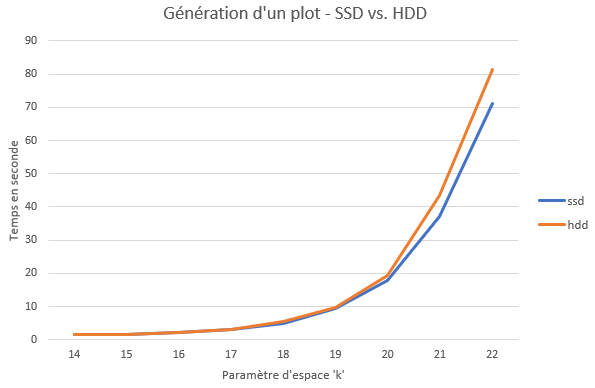
\includegraphics[width=13cm]{images/bench_ssd_hdd.png}
  \caption{Comparaison du plotting en fonction de $k$}
\end{figure}

\subsection{Comparaison du calcul des matchs}

\begin{figure}[H]
  \centering
  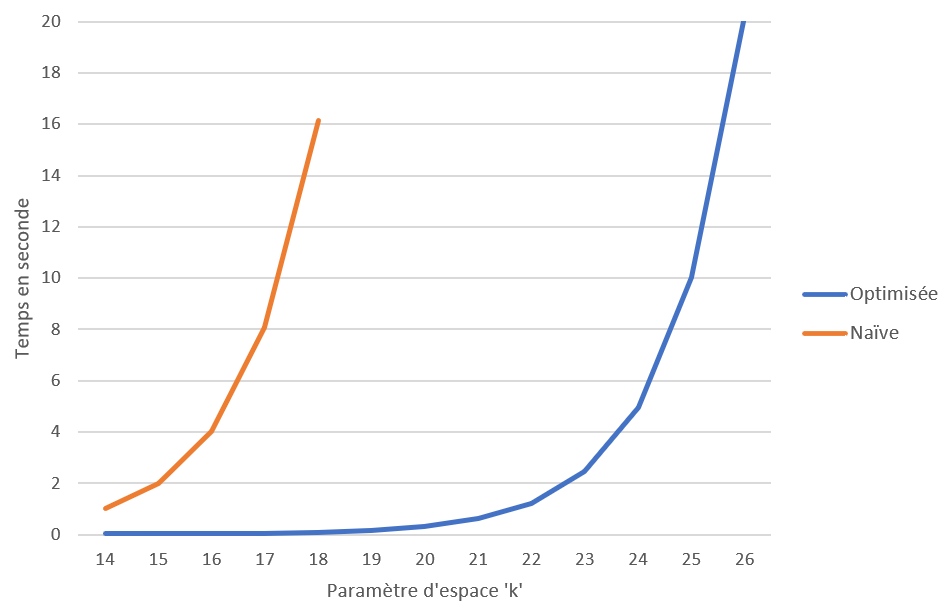
\includegraphics[width=14cm]{images/bench_matching.png}
  \caption{Comparaison des fonctions de matching en fonction de $k$}
\end{figure}

\subsection{Comparaison avec Chia}

\section{Améliorations possibles}

\lipsum[1]